\section{Final Circuit}

The final circuit design for the Low Noise Amplifier (LNA) using the BFP420 transistor is shown in Figure \ref{fig:final_circuit}. The circuit has been optimized to achieve a low noise figure and high gain at the desired frequency of 4 GHz.

\begin{figure}[H]
    \centering
    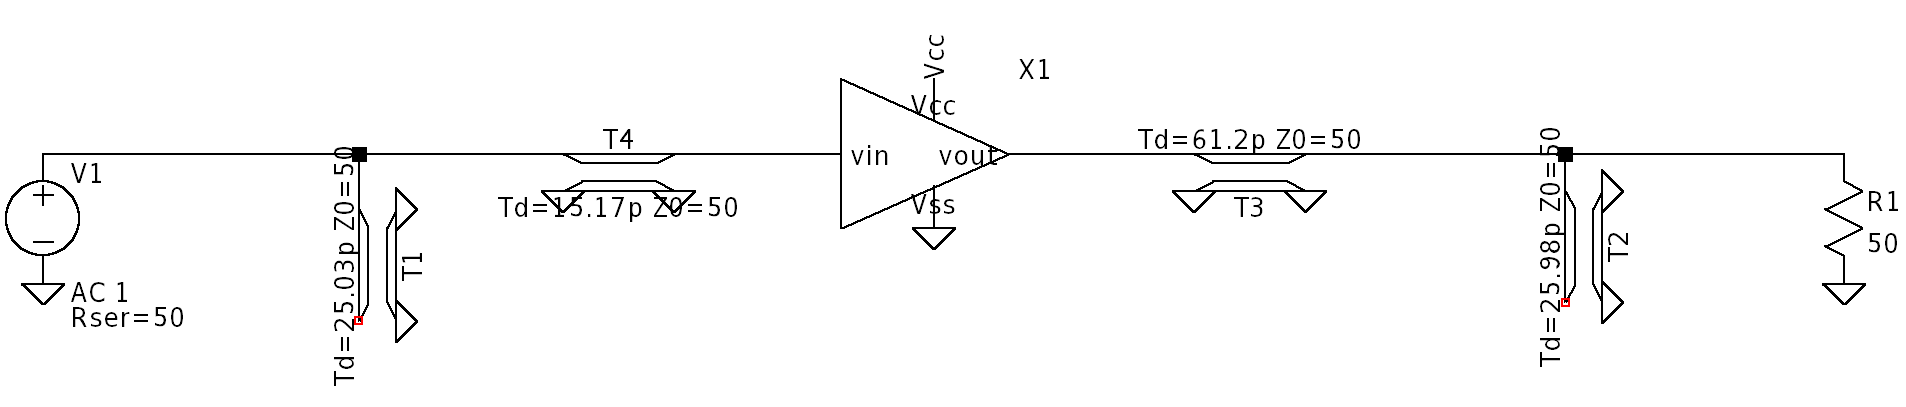
\includegraphics[width=1\textwidth]{Images/LS-gain-noise-matching-circuit.png}
    \caption{Final Circuit Design for the LNA using BFP420 Transistor.}
    \label{fig:final_circuit}
\end{figure}

The matching networks were implemented using microstrip lines due to their advantages in high-frequency performance, ease of fabrication, and seamless integration with other RF components. The design includes optimized input and output matching networks to ensure maximum power transfer while minimizing reflections. Compared to lumped components, microstrip lines offer lower parasitic effects, better power handling, and improved thermal stability. Additionally, their planar structure allows for compact routing, reduced sensitivity to manufacturing tolerances, and lower insertion losses, contributing to overall higher efficiency in the LNA design.

The final results of the circuit are shown in Table \ref{tab:final_results}, which includes the noise figure, gain, and other relevant parameters.


    \begin{table}[H]
    \centering
    \caption{Final Results of the LNA Circuit Design}
    \begin{tabularx}{\textwidth}{>{\centering\arraybackslash}X >{\centering\arraybackslash}X}
        \toprule
        \textbf{Parameter} & \textbf{Value} \\
        \midrule
        Noise Figure (NF) & 2.2 \si{\decibel} \\
        \midrule
        Gain (S21) & 13.04 \si{\decibel} \\
        \midrule
        Frequency & 4 \si{\giga \hertz} \\
        \midrule
        $I_{C}$ & 8.83 \si{\milli \ampere} \\
        \midrule
        $V_{CE}$ & 5.094 \si{\volt} \\
        \midrule
        $V_{BE}$ & 1.012 V \si{\volt}\\
        \bottomrule
    \end{tabularx}
    \label{tab:final_results}
\end{table}